\documentclass[tikz,crop,preview, border=1cm, landscape]{standalone}

\def\binOne{0.7}
\def\binTwo{0.44}
\def\binTwoStd{0.1}
\def\binOneStd{0.1}

\usepackage{pgfplots}
\pgfplotsset{compat=1.11}
\usepgfplotslibrary{fillbetween}
\usepgfplotslibrary{groupplots}

\begin{document}
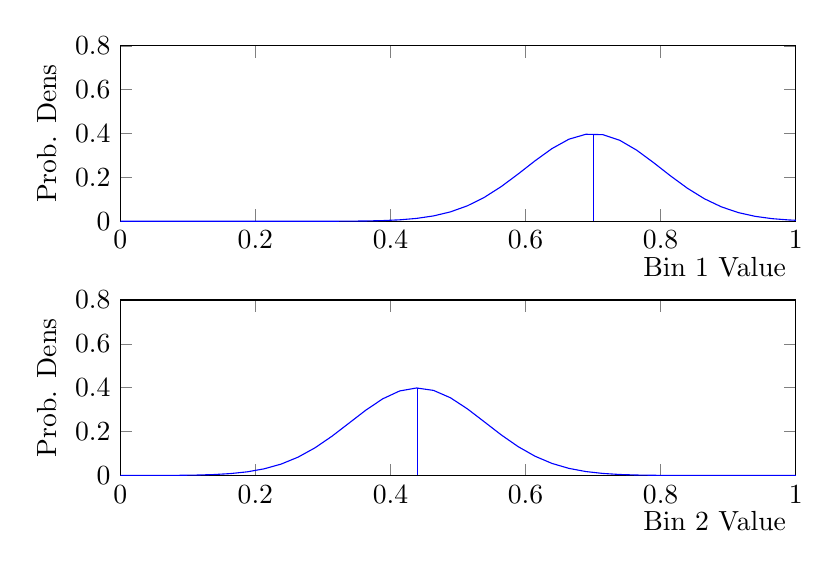
\begin{tikzpicture}
  \pgfmathdeclarefunction{gauss2}{1}{%
    \pgfmathparse{1/(\binTwoStd*sqrt(2*pi))*exp(-((#1-\binTwo)^2)/(2*\binTwoStd^2))}%
  }
  \pgfmathdeclarefunction{gauss1}{1}{%
    \pgfmathparse{1/(\binOneStd*sqrt(2*pi))*exp(-((#1-\binOne)^2)/(2*\binOneStd^2))}%
  }
  \begin{axis}[name=plot1,
    height=1.5in,
    width=4in,
    xlabel=Bin 1 Value,
    ylabel=Prob. Dens,
    ymin=0,ymax=0.8,
    xmin=0,xmax=1,
    every axis x label/.style={at={(axis description cs:1,-0.15)},anchor=north east}
    ]
    \addplot[blue, samples=400] {0.1 * gauss1(x)};
    \draw[blue] (axis cs:\binOne,0) -- (axis cs:\binOne,{0.1 * gauss1(\binOne)});
  \end{axis}
  \begin{axis}[
    name=plot2,
    at={($(plot1.south)-(0,1cm)$)},
    anchor=north,
    height=1.5in,
    width=4in,
    xlabel=Bin 2 Value,
    ylabel=Prob. Dens,
    ymin=0,ymax=0.8,
    xmin=0,xmax=1,
    x label style={at={(axis description cs:1,-0.15)},anchor=north east}
    ]
    \addplot[blue, samples=400] {0.1 * gauss2(x)};
    \draw[blue] (axis cs:\binTwo,0) -- (axis cs:\binTwo,{0.1 * gauss2(\binTwo)});
  \end{axis}
\end{tikzpicture}

\end{document}
